\documentclass{db-practice}

\usepackage{booktabs}
\usepackage{multirow}
\usepackage[nolist]{acronym}
\begin{acronym}
    \acro{FIA}{Federación Internacional de Automovilismo}
\end{acronym}

\title{Ejercicios de SQL}

\begin{document}
\maketitle

\section{Carreras de Fórmula 1}

La \ac{FIA}, como parte de su esfuerzo continuo para optimizar y mejorar la calidad de las carreras de Fórmula 1, ha tomado la decisión de recopilar y centralizar en una base de datos toda la información relevante relacionada con estos eventos de competición. Para ello, se ha diseñado una base de datos robusta y estructurada que consta de diversas tablas, las cuales tienen la función de almacenar de manera organizada toda la información referente a las carreras que se llevan a cabo durante los fines de semana en diferentes países del mundo. Estas tablas están diseñadas para capturar datos esenciales sobre cada carrera, como los equipos participantes, los pilotos, los resultados, las clasificaciones, y otros aspectos logísticos y técnicos del evento. La figura~\ref{fig:relacional} ilustra el modelo relacional de esta base de datos, proporcionando una visión clara de cómo se interconectan las diferentes tablas para ofrecer una representación integral de toda la información gestionada por la \ac{FIA} en el contexto de la Fórmula 1.

\begin{figure}[H]
  \centering
  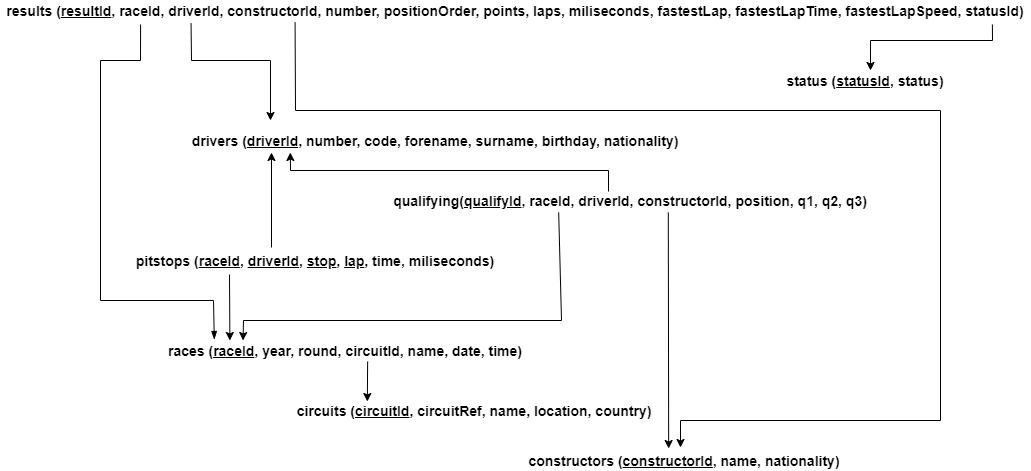
\includegraphics[width=\textwidth]{figs/modelo-relacional}
  \caption{Modelo relacional de la Fórmula 1.}
  \label{fig:relacional}
\end{figure}

A continuación se describe el contenido de las distintas tablas de la base de datos:

\begin{itemize}
    \item \texttt{drivers}: Esta tabla almacena información sobre los pilotos que han participado en las carreras, incluyendo detalles como su nombre (\texttt{forename}), apellidos (\texttt{surname}), nacionalidad (\texttt{nationality}), y otros datos relevantes para su identificación.
    \item \texttt{results}: Contiene los resultados obtenidos por cada piloto en las carreras, registrando su posición final (\texttt{positionOrder}), puntos obtenidos (\texttt{points}) y cualquier otro dato que refleje su desempeño en la competición.
    \item \texttt{races}: En esta tabla se almacena toda la información pertinente a cada carrera, como el nombre del Gran Premio (\texttt{name}), la fecha en que se disputó (\texttt{date}) y el circuito en el que tuvo lugar.
    \item \texttt{circuits}: Incluye información detallada sobre los circuitos en los que se llevan a cabo las carreras, especificando su ubicación (\texttt{location}) y nombre (\texttt{name}) entre otros.
    \item \texttt{constructors}: Esta tabla registra a los constructores (equipos) que participan en las carreras. Generalmente, cada equipo compite con dos pilotos en cada carrera.
    \item \texttt{qualifying}: Almacena los datos sobre las sesiones de calificación que determinan el orden de salida de los pilotos antes de cada carrera. Normalmente, las rondas de calificación se disputan en tres tandas (\texttt{q1}, \texttt{q2} y \texttt{q3}), en las que los pilotos más lentos van siendo eliminados sucesivamente.
    \item \texttt{pitstops}: Registra las paradas que realizan los pilotos durante las carreras, ya sea para cambiar neumáticos, repostar combustible o realizar ajustes en el coche, detallando el momento  (\texttt{lap}) y la duración de cada una (\texttt{miliseconds}).
    \item \texttt{status}: Esta tabla especifica el estado final de cada piloto al término de una carrera, indicando si finalizaron en condiciones normales, si perdieron vueltas, si tuvieron problemas técnicos o si abandonaron por alguna razón.
\end{itemize}

Adicionalmente, se hace constar que este modelo tiene añadidas las siguientes restricciones:

\begin{itemize}
    \item Todos los identificadores se presentan de forma numérica.
    \item Los nombres, apellidos, nacionalidades y localizaciones no podrán exceder en ningún caso los 250 caracteres.
    \item Los campos que indican número de vuelta, puntos y velocidades tendrán que adaptarse como valores \texttt{INT}, \texttt{FLOAT} o \texttt{DOUBLE} según corresponda.
    \item Existen tres tipos adicionales de valores con formato temporal como son \textit{time} de tipo \texttt{TIME}, \textit{date} y \textit{birthday} de tipo \texttt{DATE} y \textit{year} de tipo \texttt{YEAR}.
\end{itemize}

\subsection{Consultas SQL:}

\begin{enumerate}
    \item Obtener el nombre y apellidos de los pilotos españoles.

    \item Obtener todos los datos de los circuitos alemanes.
    
    \item Obtener los paises en los que se disputaron carreras en el año 2010.

    \item Obtener el nombre de los pilotos que han participado en al menos 1 carrera del año 2016.

    \item Nombre de los constructores con los que han disputado carreras más de 50 pilotos diferentes.
    
    \item Nombre y apellidos de los pilotos que nunca han ganado una carrera.
              
    \item Obtener el nombre y apellidos de los pilotos que durante el año 2017 han participado en todas las carreras.
    
    \item Obtener el nombre, localización, país y año para cada circuito de las carreras que se han disputado entre 2015 y 2017, ordenado por el id del circuito.
    
    \item Obtener los constructores que no han participado en alguna clasificación.
              
    \item Obtener nombres, apellidos de los pilotos que han ganado más de 30 grandes premios así como el número de grandes premios que han ganado.
       
    \item Nombre y apellidos del piloto que obtuvo la vuelta con velocidad media más alta así como el circuito y el año en el que se obtuvo.
    
    \item Obtener el nombre, apellidos y la velocidad media del piloto que obtuvo la vuelta con velocidad media más alta en el gran premio de Japón de 2009.
             
    \item Obtener el nombre de los pilotos que durante el año 2017 consiguieron puntos en todas las carreras.
    
    \item Obtener el nombre de los pilotos, el circuito y el total de paradas, para aquellos pilotos que entre todos los grandes premios disputados han realizado en alguno de ellos el mayor número de paradas y también los que han realizado el menor número de ellas.
      
    \item De entre todos los pilotos que han participado en todas las rondas de clasificación (Q1, Q2 y Q3) del gran premio de Abu Dhabi de 2017 (\texttt{qualifying.q1 <> '' AND qualifying.q2 <> '' AND qualifying.q3 <> ''}), obtener el nombre de los pilotos y el id de los equipos, para aquellos equipos que tienen a sus dos pilotos en esa situación.
    
    \item Obtener el nombre y apellido de los pilotos y el nombre de aquellas carreras en las que han participado pilotos rusos y polacos.
            
    \item Obtener el nombre y apellidos de los pilotos y el número de vueltas totales recorridas en el año 2011 siempre y cuando sea mayor que la media del número de vueltas totales recorridas el año anterior por todos los pilotos.

    \item Obtener el nombre y año de las carreras en las que se disputó una clasificación (\texttt{qualifying}) pero no se realizaron pitstops.
    
    \item Obtener la nacionalidad de los pilotos que han disputado todas las ediciones del gran premio `Australian Grand Prix'.
    
    \item Eliminar de la tabla \texttt{qualifying} aquellas tuplas donde un piloto no haya participado en la clasificación.
            
    \item Obtener aquellos constructores que habiendo ganado más de 5 carreras entre 2003 y 2010, no hayan participado en ninguna carrera desde el siguiente año.
    
    \item Obtener el nombre de la carrera y el año en la que tuvo lugar todos los tipos de incidentes que se enumeran a continuación: descalificación, accidente, colisión, fallo de motor, caja de cambios y transmisión (\texttt{statusId} de 2 a 7).
    
    \item Obtener nombre y apellidos del piloto, el nombre del circuito, el año de la carrera donde un piloto español obtuvo el tiempo de parada más pequeño (atributo \texttt{miliseconds}). Incluya este atributo en la salida de la consulta.

    \item Codifique una consulta que obtenga el nombre de aquellos constructores que sean italianos (\texttt{nationality = 'Italian'}) con los que hayan disputado carreras al menos un piloto italiano.
            
    \item Codifique una consulta que obtenga el nombre y apellidos del piloto que más accidentes (\texttt{status.status = `Accident'}) ha tenido. Mostrar también el número de accidentes.
            
    \item Codifique una consulta que obtenga el nombre y apellidos de los pilotos que hayan calificado entre los 10 primeros puestos (\texttt{position <= 10}) de todas las carreras del año 2015.
    
    \item Obtener una lista con los nombres de aquellos constructores italianos (‘Italian’ en inglés) que nunca han competido con pilotos italianos.
    
    \item Obtener toda la información de los constructores que en todas las carreras del año 2006, consiguieron que alguno de sus pilotos quedara entre los diez primeros de la clasificación.
    
    \item Obtener nombre y apellidos del piloto que acabó la competición con más puntos entre los años 1990 y 2000, así como dicha suma de puntos.

    \item Codifique una consulta que obtenga el nombre y apellidos de los pilotos que ganaron una carrera (\texttt{results.positionOrder = 1}) sin haber estado clasificados entre los 10 primeros pilotos (\texttt{qualifying.position > 10}). Mostrar además el nombre de la carrera y el año en la que lo consiguieron.

    \item Codifique una consulta que obtenga el nombre y apellidos del piloto que realizó más \emph{pitstops} en una carrera del año 2013. Mostrar también el número de \emph{pitstops}.
    
    \item Codifique una consulta que obtenga el nombre y apellidos de los pilotos que hayan quedado entre los 10 primeros puestos (\texttt{positionOrder <= 10}) de todas las carreras del año 2017.
\end{enumerate}

\subsection{Procedimientos almacenados:}

\begin{enumerate}
    \item Crea un procedimiento almacenado de nombre \texttt{getRacesInAYear}, que obtenga como salida los nombres de las carreras y el número total de constructores que han participado en la carrera, para un año concreto que se pasará como parámetro de entrada. En el procedimiento no se definirán parámetros de salida.  
        
    \item Se quiere testear los mensajes que se le envían a los pilotos por pantalla en plena carrera. Para ello se quiere crear un procedimiento de nombre \texttt{getOnRaceMessages}, que reciba un código de mensaje, e indique en un parámetro de salida el mensaje concreto teniendo en cuenta las siguientes condiciones:
    \begin{itemize}
        \item E01 = Error en la presión de las ruedas
        \item E02 = Pinchazo
        \item E03 = Temperatura alta en el motor
        \item E04 = Frenos sobre-calentados
        \item E05 = Error presión del aceite
        \item Cualquier otro valor = Error de comando
    \end{itemize} 

    \item Crea un procedimiento almacenado para obtener los pilotos y los circuitos que ganaron carreras de un año concreto (como argumento) con un constructor del mismo país que el piloto.

    \item Escribe un procedimiento que realice la selección de aquellos pilotos que en el año que se le pase como parámetro de entrada, obtuvieron un primer, un segundo y un tercer puesto.
    
    \item Procedimiento almacenado de nombre \texttt{getsConstructoresYPilotos}, que tomando como entrada un año concreto, obtenga como salida los nombres de todos los pilotos que participaron en el mundial ese año y el equipo de constructores con el cual compitieron. Adicionalmente, también se quiere obtener el total de puntos que obtuvo cada piloto en el mundial.

    \item Codifique un procedimiento almacenado denominado \texttt{getNumberOfVictories} que disponga de un parámetro de entrada \texttt{type}. Si \texttt{type = 'nationality'}, el procedimiento listará el número de victorias que han obtenido cada una de las nacionalidades de la tabla \texttt{drivers}. Por contra, si \texttt{type} toma cualquier otro valor, el procedimiento listará el número de victorias que han obtenidos cada uno de los constructores (\texttt{constructors.name}) existentes en la base de datos. Los resultados deberá estar ordenados de mayor a menor número de victorias.
    
    \item Añade una nueva columna en la tabla \texttt{drivers} que se llame años en activo. A continuación escribir un procedimiento que, haciendo uso de un \texttt{Cursor}, calcule el número total de años que ha estado un piloto compitiendo y actualice la tabla.

    \item Crea un procedimiento que reciba una nacionalidad como parámetro de entrada y realice una consulta sobre la tabla \texttt{drivers} para obtener todos los pilotos de esa nacionalidad. Los nombres y apellidos de estos pilotos deberán devolverse en un parámetro de salida de tipo \texttt{TEXT} separados por comas (\texttt{,}).
\end{enumerate}


\subsection{Funciones almacenadas:}

\begin{enumerate}
    \item Escribe una función que devuelva el número de puntos que se ha conseguido el campeón de ese año en cada mundial.
       
    \item Escribe una función que devuelva el valor medio de puntos por año que ha conseguido un determinado constructor que se recibirá como parámetro de entrada. El parámetro de entrada será el nombre del constructor.
            
    \item Escribe una función que dado el \texttt{driverId} de un piloto devuelva el número total de años en activo que ha estado compitiendo.

    \item Codifique una función almacenada llamada \texttt{diffPoints} que reciba los identificadores de dos pilotos como parámetros (\texttt{driver1} y \texttt{driver2}) y devuelva la diferencia de puntos totales conseguidos por \texttt{driver1} con respecto de \texttt{driver2}. Tenga en cuenta que el valor será positivo si \texttt{driver1} ha conseguido más puntos que \texttt{driver2} y negativo en caso contrario.
\end{enumerate}

\subsection{Triggers:}

\begin{enumerate}
    %\item A partir de este momento la FIA no va a permitir que haya equipos con más de 2 pilotos, por ello se debe desarrollar un trigger que impida que se puedan incorporar en un mismo equipo más de 2 pilotos a la base de datos. Para ello, se debe impedir toda operación que haga que 3 o más pilotos pasen a formar parte del mismo equipo de constructores, ya sea mediante inserción o actualización de los datos. 
    
    \item Desarrolle taodos los triggers necesarios para impedir que en una misma carrera no puedan participar más de 2 pilotos con un constructor. Se considera que participar en una carrera es aparecer en la tabla \texttt{results} (se ignora por tanto la tabla \texttt{qualifying}).
        
    \item Crea una tabla \texttt{crashes} con la siguiente estructura:
    \begin{table}[H]
    \centering
    \begin{tabular}{@{}lll@{}}
    \toprule
    \multicolumn{1}{c}{\textbf{crashId}} & \multicolumn{1}{c}{\textbf{driverId}} & \multicolumn{1}{c}{\textbf{descripción}} \\ \midrule
                                         &                                       &                                          \\ \bottomrule
    \end{tabular}
    \end{table}

    Crea un trigger que cuando se inserte una fila en la tabla \texttt{results} con el parámetro \texttt{statusId} de valores 3 ó 4 rellene la tabla \texttt{crashes} con la información correspondiente.

    \item Crea un trigger para impedir que en un mismo año un piloto participe en carreras con dos constructores diferentes. Se considera que un piloto habrá participado en una carrera si aparece en la tabla \texttt{results}.
    
    \item Cree una nueva tabla \textit{sponsors} en la base de datos que almacene como atributos, su identificador propio, su nombre, tipo, el identificador de la carrera que patrocina (un patrocinador solo puede patrocinar una carrera) y el dinero que aporta anualmente. Existen dos tipos de patrocinadores: oficiales, deben aportan una cantidad igual o superior a 5M de euros, y cooficiales, para cantidades inferiores. Diseñe un trigger que clasifique al sponsor y rellene el atributo \textit{type} de su correspondiente tabla.
    
    %\item A partir de ahora, los patrocinadores van a poder patrocinar varias carreras. Realize las modificaciones que considere necesarias en el \texttt{schema} de la base de datos y actualice los triggers para garantizar que el tipo de patrocinador sea siempre correcto.
\end{enumerate}

\section{Soluciones}

\subsection{Consultas SQL}

\begin{enumerate}

% Obtener el nombre y apellidos de los pilotos españoles.
\item 
\begin{lstlisting}[language=SQL]
SELECT surname, forename
FROM drivers 
WHERE nationality = "Spanish"
\end{lstlisting}

% Obtener todos los datos de los circuitos alemanes.
\item 
\begin{lstlisting}[language=SQL]
SELECT *
FROM circuits 
WHERE country = "Germany"
\end{lstlisting}

% Obtener los paises en los que se disputaron carreras en el año 2010.
\item
\begin{lstlisting}[language=SQL]
SELECT DISTINCT country
FROM circuits
    INNER JOIN races ON races.circuitId = circuits.circuitId
WHERE year = 2010
\end{lstlisting}

% Obtener el nombre de los pilotos que han participado en al menos 1 carrera del año 2016.
\item
\begin{lstlisting}[language=SQL]
SELECT DISTINCT drivers.surname, drivers.forename
FROM drivers 
    INNER JOIN results ON drivers.driverId = results.driverId
    INNER JOIN races ON results.raceId = races.raceId
WHERE year = 2016
\end{lstlisting}

% Nombre de los constructores con los que han disputado carreras mas de 50 pilotos diferentes.
\item
\begin{lstlisting}[language=SQL]
SELECT name
FROM constructors
WHERE constructorId IN (SELECT constructorId
                        FROM results
                        GROUP BY constructorId
                        HAVING COUNT(DISTINCT driverId) > 50)
\end{lstlisting}

% Nombre y apellidos de los pilotos que nunca han ganado una carrera.
\item
\begin{lstlisting}[language=SQL]
SELECT forename, surname
FROM drivers
WHERE driverId NOT IN (SELECT driverId
                FROM results
                WHERE positionOrder = 1)
\end{lstlisting}
         
% Obtener el nombre y apellidos de los pilotos que durante el año 2017 han participado en todas las carreras.
\item
\begin{lstlisting}[language=SQL]
SELECT drivers.surname, drivers.forename
FROM drivers
WHERE driverId IN (SELECT driverId
                   FROM results
                   WHERE raceId IN (SELECT raceId FROM races WHERE year=2017)
                   GROUP BY results.driverId
                   HAVING COUNT(distinct results.raceId) = (SELECT COUNT(*)
                                                            FROM races
                                                            WHERE year=2017))
\end{lstlisting}

% Obtener el nombre, localizacion, pais y año para cada circuito de las carreras que se han disputado entre 2015 y 2017, ordenado por el id del circuito.
\item
\begin{lstlisting}[language=SQL]
SELECT circuits.circuitId, circuits.name, circuits.location, circuits.country, year
FROM races 
    INNER JOIN circuits ON races.circuitId = circuits.circuitId
WHERE year BETWEEN 2015 AND 2017
ORDER BY circuits.circuitId
\end{lstlisting}

% Obtener los constructores que no han participado en alguna clasificación.
\item
\begin{lstlisting}[language=SQL]
SELECT *
FROM constructors
WHERE constructors.constructorId NOT IN (SELECT qualifying.constructorId 
                                         FROM qualifying)  
\end{lstlisting}
        
% Obtener nombres, apellidos de los pilotos que han ganado más de 30 grandes premios así como el número de grandes premios que han ganado.
\item
\begin{lstlisting}[language=SQL]
SELECT drivers.surname, drivers.forename, COUNT(*) AS wins
FROM drivers
    INNER JOIN results ON results.driverId = drivers.driverId
WHERE positionOrder = 1
GROUP BY drivers.driverId, drivers.surname, drivers.forename
HAVING COUNT(*) >= 30
\end{lstlisting}

% Nombre y apellidos del piloto que obtuvo la vuelta con velocidad media más alta así como el circuito y el año en el que se obtuvo.
\item
\begin{lstlisting}[language=SQL]
SELECT drivers.forename, drivers.surname, circuits.name, races.year, results.fastestLapSpeed
FROM drivers
    INNER JOIN results ON drivers.driverId = results.driverId
    INNER JOIN races ON races.raceId = results.raceId
    INNER JOIN circuits ON circuits.circuitId = races.circuitId
WHERE fastestLapSpeed >= ALL (SELECT fastestLapSpeed
                              FROM results)
\end{lstlisting}

% Obtener el nombre, apellidos y la velocidad media del piloto que obtuvo la vuelta con velocidad media más alta en el gran premio de Japón de 2009.
\item
\begin{lstlisting}[language=SQL]
SELECT drivers.forename, drivers.surname, results.fastestLapSpeed
FROM drivers
    INNER JOIN results ON results.driverId = drivers.driverId
    INNER JOIN races ON races.raceId = results.raceId
WHERE races.year = 2009
    AND races.name = 'Japanese Grand Prix'
    AND results.fastestLapSpeed >= ALL (SELECT fastestLapSpeed
                                        FROM results
                                        INNER JOIN races ON races.raceId = results.raceId
                                        WHERE year = 2009
                                        AND name = 'Japanese Grand Prix')
\end{lstlisting}
        
% Obtener el nombre de los pilotos que durante el año 2017 consiguieron puntos en todas las carreras.
\item
\begin{lstlisting}[language=SQL]
SELECT drivers.forename, drivers.surname
FROM results
    INNER JOIN races ON races.raceId = results.raceId
    INNER JOIN drivers ON drivers.driverId = results.driverId
WHERE points > 0
    AND year = 2017
GROUP BY drivers.driverId, drivers.forename, drivers.surname
HAVING COUNT(*) = (SELECT COUNT(*)
                   FROM races
                   WHERE year = 2017)
\end{lstlisting}

% Obtener el nombre de los pilotos, el circuito y el total de paradas, para aquellos pilotos que entre todos los grandes premios disputados han realizado en alguno de ellos el mayor número de paradas y también los que han realizado el menor número de ellas.
\item
\begin{lstlisting}[language=SQL]
SELECT drivers.forename, drivers.surname, circuits.name, races.year, COUNT(*)
FROM drivers
    INNER JOIN pitstops ON pitstops.driverId = drivers.driverId
    INNER JOIN races ON races.raceId = pitstops.raceId
    INNER JOIN circuits ON circuits.circuitId = races.circuitId
GROUP BY drivers.driverId, drivers.forename, drivers.surname, races.raceId, races.year, circuits.name
HAVING COUNT(*) >= ALL(SELECT COUNT(*)
                       FROM pitstops
                       GROUP BY driverId, raceId)
\end{lstlisting}
 
% De entre todos los pilotos que han participado en todas las rondas de clasificación (Q1, Q2 y Q3) del gran premio de Abu Dhabi de 2017 (\texttt{qualifying.q1 <> '' AND qualifying.q2 <> '' AND qualifying.q3 <> ''}), obtener el nombre de los pilotos y el id de los equipos, para aquellos equipos que tienen a sus dos pilotos en esa situación.
\item
\begin{lstlisting}[language=SQL]
SELECT drivers.forename, drivers.surname, constructors.name
FROM drivers
    INNER JOIN qualifying ON qualifying.driverId = drivers.driverId
    INNER JOIN constructors ON qualifying.constructorId = constructors.constructorId
    INNER JOIN races ON races.raceId = qualifying.raceId
WHERE races.year = 2017
    AND races.name = 'Abu Dhabi Grand Prix'
    AND constructors.constructorId IN (SELECT qualifying.constructorId
                                       FROM qualifying
                                           INNER JOIN races ON races.raceId = qualifying.raceId
                                       WHERE races.year = 2017
                                         AND races.name = 'Abu Dhabi Grand Prix'
                                         AND qualifying.q1 <> ''
                                         AND qualifying.q2 <> ''
                                         AND qualifying.q3 <> ''
                                       GROUP BY qualifying.constructorId
                                       HAVING COUNT(DISTINCT qualifying.driverId) = 2)
ORDER BY constructors.name ASC
\end{lstlisting}

% Obtener el nombre y apellido de los pilotos y el nombre de aquellas carreras en las que han participado pilotos rusos y polacos.
\item
\begin{lstlisting}[language=SQL]
SELECT drivers.forename, drivers.surname, races.name, races.year
FROM drivers
    INNER JOIN results ON results.driverId = drivers.driverId
    INNER JOIN races ON races.raceId = results.raceId
WHERE races.raceId IN (SELECT raceId
                       FROM results 
                           INNER JOIN drivers ON drivers.driverId = results.driverId
                       WHERE drivers.nationality = "Russian")
  AND races.raceId IN (SELECT raceId
                       FROM results 
                           INNER JOIN drivers ON drivers.driverId = results.driverId
                       WHERE drivers.nationality = "Polish")
\end{lstlisting}
      
% Obtener el nombre y apellidos de los pilotos y el número de vueltas totales recorridas en el año 2011 siempre y cuando sea mayor que la media del número de vueltas totales recorridas el año anterior por todos los pilotos.
\item
\begin{lstlisting}[language=SQL]
SELECT drivers.forename, drivers.surname, SUM(results.laps)
FROM drivers
    INNER JOIN results ON results.driverId = drivers.driverId
    INNER JOIN races ON races.raceId = results.raceId
WHERE races.year = 2011
GROUP BY drivers.driverId, drivers.forename, drivers.surname
HAVING SUM(results.laps) > (SELECT AVG(nLaps)
                            FROM (SELECT SUM(laps) AS nLaps
                                    FROM results
                                        INNER JOIN races ON races.raceId = results.raceId
                                    WHERE year = 2010
                                    GROUP BY driverId) t)
\end{lstlisting}

% Obtener el nombre y año de las carreras en las que se disputó una clasificación (\texttt{qualifying}) pero no se realizaron pitstops.
\item
\begin{lstlisting}[language=SQL]
SELECT name, year
FROM races
WHERE raceId IN (SELECT raceId FROM qualifying)
  AND raceId NOT IN (SELECT raceId FROM pitstops)
\end{lstlisting}

% Obtener la nacionalidad de los pilotos que han disputado todas las ediciones del gran premio `Australian Grand Prix'.
\item
\begin{lstlisting}[language=SQL]
SELECT drivers.nationality
FROM drivers
    INNER JOIN results ON results.driverId = drivers.driverId
    INNER JOIN races ON races.raceId = results.raceId
WHERE races.name = "Australian Grand Prix"
GROUP BY drivers.driverId, drivers.nationality
HAVING COUNT(*) = (SELECT COUNT(*)
                   FROM races
                   WHERE name = "Australian Grand Prix")
\end{lstlisting}

% Eliminar de la tabla \texttt{qualifying} aquellas tuplas donde un piloto no haya participado en la clasificación.
\item
\begin{lstlisting}[language=SQL]
DELETE FROM qualifying
WHERE q1 = '' AND q2 = '' AND q3 = ''
\end{lstlisting}
       
% Obtener aquellos constructores que habiendo ganado más de 5 carreras entre 2003 y 2010, no hayan participado en ninguna carrera desde el siguiente año.
\item
\begin{lstlisting}[language=SQL]
SELECT *
FROM constructors
WHERE constructorId IN (SELECT results.constructorId
                        FROM results
                            INNER JOIN races ON races.raceId = results.raceId
                        WHERE races.year BETWEEN 2003 AND 2010
                          AND results.positionOrder = 1
                        GROUP BY results.constructorId
                        HAVING COUNT(*) > 5)
  AND constructorId NOT IN (SELECT results.constructorId
                            FROM results
                                INNER JOIN races ON races.raceId = results.raceId
                            WHERE races.year > 2010)
\end{lstlisting}

% Obtener el nombre de la carrera y el año en la que tuvo lugar todos los tipos de incidentes que se enumeran a continuación: descalificación, accidente, colisión, fallo de motor, caja de cambios y transmisión (\texttt{statusId} de 2 a 7).
\item
\begin{lstlisting}[language=SQL]
SELECT races.raceId, races.name, races.year, COUNT(DISTINCT results.statusId)
FROM races
    INNER JOIN results ON results.raceId = races.raceId
WHERE results.statusId BETWEEN 2 AND 7
GROUP BY races.raceId, races.name, races.year
HAVING COUNT(DISTINCT results.statusId) = (SELECT COUNT(*)
                                           FROM status
                                           WHERE statusId BETWEEN 2 AND 7)
\end{lstlisting}

% Obtener nombre y apellidos del piloto, el nombre del circuito, el año de la carrera donde un piloto español obtuvo el tiempo de parada más pequeño (atributo \texttt{miliseconds}). Incluya este atributo en la salida de la consulta.
\item
\begin{lstlisting}[language=SQL]
SELECT forename, surname, circuits.name, races.year, miliseconds
FROM drivers, pitstops, races, circuits
WHERE drivers.driverId=pitstops.driverId 
  AND pitstops.raceId=races.raceId
  AND races.circuitId=circuits.circuitId
  AND drivers.nationality='Spanish'
  AND miliseconds = (SELECT MIN(miliseconds)
                     FROM pitstops JOIN drivers ON pitstops.driverId=drivers.driverId
                     WHERE drivers.nationality='Spanish');
\end{lstlisting}

% Codifique una consulta que obtenga el nombre de aquellos constructores que sean italianos (\texttt{nationality = 'Italian'}) con los que hayan disputado carreras al menos un piloto italiano.
\item
\begin{lstlisting}[language=SQL]
SELECT DISTINCT name
FROM constructors
    INNER JOIN results ON results.constructorId = constructors.constructorId
    INNER JOIN drivers ON drivers.driverId = results.resultId
WHERE constructors.nationality LIKE 'Italian'
  AND drivers.nationality LIKE 'Italian'
\end{lstlisting}
       
% Codifique una consulta que obtenga el nombre y apellidos del piloto que más accidentes (\texttt{status.status = `Accident'}) ha tenido. Mostrar también el número de accidentes.
\item
\begin{lstlisting}[language=SQL]
SELECT drivers.forename, drivers.forename, COUNT(*)
FROM drivers
    INNER JOIN results ON results.driverId = drivers.driverId
    INNER JOIN status ON status.statusId = results.statusId
WHERE status.status LIKE 'Accident'
GROUP BY drivers.driverId, drivers.forename, drivers.surname
HAVING COUNT(*) >= ALL (SELECT COUNT(*)
                        FROM results
                            INNER JOIN status ON status.statusId = results.statusId
                        WHERE status.status LIKE 'Accident'
                        GROUP BY results.driverId) 
\end{lstlisting}
      
% Codifique una consulta que obtenga el nombre y apellidos de los pilotos que hayan calificado entre los 10 primeros puestos (\texttt{position <= 10}) de todas las carreras del año 2015.
\item
\begin{lstlisting}[language=SQL]
SELECT drivers.forename, drivers.surname
FROM drivers 
    INNER JOIN qualifying ON qualifying.driverId = drivers.driverId
    INNER JOIN races ON races.raceId = qualifying.raceId
WHERE position <= 10
  AND year = 2015
GROUO BY drivers.driverId, drivers.forename, drivers.surname
HAVING COUNT(*) = (SELECT COUNT(*) FROM races WHERE year = 2015);
\end{lstlisting}

% Obtener una lista con los nombres de aquellos constructores italianos (‘Italian’ en inglés) que nunca han competido con pilotos italianos.
\item
\begin{lstlisting}[language=SQL]
SELECT name
FROM constructors
WHERE constructorId NOT IN (SELECT constructorId
                            FROM results JOIN drivers ON results.driverId=drivers.driverId
                            WHERE nationality='Italian')
AND nationality='Italian';
\end{lstlisting}

% Obtener toda la información de los constructores que en todas las carreras del año 2006, consiguieron que alguno de sus pilotos quedara entre los diez primeros de la clasificación.
\item
\begin{lstlisting}[language=SQL]
SELECT constructors.*
FROM constructors 
    INNER JOIN qualifying ON qualifying.constructorId = constructors.constructorId
    INNER JOIN races ON races.raceId = qualifying.raceId
WHERE position <= 10
    AND year = 2006
GROUO BY constructors.constructorId
HAVING COUNT(DISTINCT raceId) = (SELECT COUNT(*) FROM races WHERE year = 2006);
\end{lstlisting}

% Obtener nombre y apellidos del piloto que acabó la competición con más puntos entre los años 1990 y 2000, así como dicha suma de puntos.
\item
\begin{lstlisting}[language=SQL]
SELECT forename, surname, suma
FROM(SELECT driverId, year, SUM(points) as suma
        FROM results JOIN races ON results.raceId=races.raceId
        WHERE year BETWEEN 1990 AND 2000
        GROUP BY driverId, year
        HAVING SUM(points)>0) AS puntuaciones
JOIN drivers ON puntuaciones.driverId=drivers.driverId
WHERE suma >= ALL (SELECT SUM(points)
                    FROM results JOIN races ON results.raceId=races.raceId
                    WHERE year BETWEEN 1990 AND 2000
                    GROUP BY driverId, year
                    HAVING SUM(points)>0)
\end{lstlisting}

% Codifique una consulta que obtenga el nombre y apellidos de los pilotos que ganaron una carrera (\texttt{results.positionOrder = 1}) sin haber estado clasificados entre los 10 primeros pilotos (\texttt{qualifying.position > 10}). Mostrar además el nombre de la carrera y el año en la que lo consiguieron.
\item
\begin{lstlisting}[language=SQL]
SELECT DISTINCT drivers.forename, drivers.surname, races.name, races.year
FROM drivers
    INNER JOIN results ON results.driverId = drivers.driverId
    INNER JOIN races ON races.raceId = results.raceId
WHERE results.positionOrder = 1
  AND driverId IN (SELECT driverId
                   FROM qualifying
                   WHERE qualifying.raceId = races.raceId
                     AND position > 10)
\end{lstlisting}

% Codifique una consulta que obtenga el nombre y apellidos del piloto que realizó más \emph{pitstops} en una carrera del año 2013. Mostrar también el número de \emph{pitstops}.
\item
\begin{lstlisting}[language=SQL]
SELECT drivers.forename, drivers.surname, COUNT(*)
FROM drivers
    INNER JOIN pitstops ON pitstops.driverId = drivers.driverId
    INNER JOIN races ON races.raceId = pitstops.raceId
WHERE races.year = 2013
GROUP BY pitstops.driverId, pitstops.raceId, drivers.forename, drivers.surname
HAVING COUNT(*) >= ALL (SELECT COUNT(*)
                        FROM pitstops
                        GROUP BY pitstops.driverId, pitstops.raceId)  
\end{lstlisting}

% Codifique una consulta que obtenga el nombre y apellidos de los pilotos que hayan quedado entre los 10 primeros puestos (\texttt{positionOrder <= 10}) de todas las carreras del año 2017.
\item
\begin{lstlisting}[language=SQL]
SELECT drivers.forename, drivers.surname
FROM drivers 
    INNER JOIN results ON results.driverId = drivers.driverId
    INNER JOIN races ON races.raceId = results.raceId
WHERE year = 2017
  AND positionOrder <= 10
GROUP BY drivers.driverId, drivers.forename, drivers.surname
HAVING COUNT(*) = (SELECT COUNT(*) FROM races WHERE year = 2017)
\end{lstlisting}

\end{enumerate}

\subsection{Procedimientos almacenados:}

\begin{enumerate}

\item
\begin{lstlisting}[language=SQL]
DELIMITER $$
CREATE PROCEDURE `getRacesInAYear`(IN `year` INTEGER)
BEGIN
	SELECT races.name, COUNT(DISTINCT results.constructorId) AS numConstructors
    FROM results
    	INNER JOIN races ON races.raceId = results.raceId
    WHERE races.year = year
    GROUP BY races.raceId;
END$$
DELIMITER ;
\end{lstlisting}

\item
\begin{lstlisting}[language=SQL]
DELIMITER $$
CREATE PROCEDURE getsOnRaceMessages(IN cod VARCHAR(3), OUT msg VARCHAR(200))
BEGIN
    CASE cod
    WHEN 'E01' THEN SET msg = 'Error en la presion de las ruedas';
    WHEN 'E02' THEN SET msg = 'Pinchazo';
    WHEN 'E03' THEN SET msg = 'Temperatura alta en el motor';
    WHEN 'E04' THEN SET msg = 'Frenos sobre-calentados';
    WHEN 'E05' THEN SET msg = 'Error presion del aceite';
    ELSE SET msg = 'Error de comando';
    END CASE;
END$$
DELIMITER ;
\end{lstlisting}

\item
\begin{lstlisting}[language=SQL]
DELIMITER $$
CREATE PROCEDURE driversWinningAtHome (IN year_win INTEGER)
BEGIN
    SELECT DISTINCT drivers.forename, drivers.surname, circuits.name
    FROM drivers INNER JOIN results ON drivers.driverId = results.driverId INNER JOIN races ON results.raceId=races.raceId INNER JOIN constructors ON results.constructorId=constructors.constructorId INNER JOIN circuits ON circuits.circuitId=races.circuitId 
    WHERE results.positionOrder=1 AND races.year=year_win AND drivers.nationality=constructors.nationality;
END$$
DELIMITER ;
\end{lstlisting}

\item
\begin{lstlisting}[language=SQL]
DELIMITER $$
CREATE PROCEDURE allPodiumPositions(IN anyo INTEGER)
BEGIN
SELECT forename, surname
FROM drivers D
WHERE driverId IN(SELECT driverId
                  FROM results JOIN races ON results.raceId=races.raceId
                  WHERE positionOrder=1
                    AND year=anyo)
  AND driverId IN(SELECT driverId
                  FROM results JOIN races ON results.raceId=races.raceId
                  WHERE positionOrder=2
                    AND year=anyo)
  AND driverId IN(SELECT driverId
                  FROM results JOIN races ON results.raceId=races.raceId
                  WHERE positionOrder=3
                    AND year=anyo);
END$$ 
DELIMITER ;  
\end{lstlisting}

\item
\begin{lstlisting}[language=SQL]
DELIMITER $$
CREATE PROCEDURE getsConstructoresYPilotos (IN año YEAR)
BEGIN
    SELECT constructors.name, drivers.surname, SUM(results.points)
    FROM constructors JOIN results ON constructors.constructorId = results.constructorID
        JOIN races ON results.raceId = races.raceId
        JOIN drivers ON results.driverId = drivers.driverId
    WHERE races.year= año
    GROUP BY constructors.name, drivers.surname;
END$$ 
DELIMITER ;
\end{lstlisting}

\item
\begin{lstlisting}[language=SQL]
DELIMITER $$
CREATE PROCEDURE getNumberOfVictories (IN type VARCHAR(20)) 
BEGIN
    IF type = 'nationality' THEN
        SELECT drivers.nationality, COUNT(*) AS numVictorires
        FROM results
            INNER JOIN drivers ON drivers.driverId = results.driverId
        WHERE results.positionOrder = 1
        GROUP BY drivers.nationality
        ORDER BY numVictorires DESC;
    ELSE 
        SELECT constructors.name, COUNT(*) AS numVictorires
        FROM results
            INNER JOIN constructors ON constructors.constructorId = results.constructorId
        WHERE results.positionOrder = 1
        GROUP BY constructors.name
        ORDER BY numVictorires DESC;
    END IF;
END$$
DELIMITER ;  
\end{lstlisting}

\item
\begin{lstlisting}[language=SQL]
ALTER TABLE drivers ADD COLUMN añosEnActivo INTEGER NULL;

DELIMITER $$
CREATE PROCEDURE actualizarAñosEnActivo ()
BEGIN
    DECLARE done INTEGER DEFAULT FALSE;
    DECLARE id INTEGER;
    
    DECLARE cur CURSOR FOR SELECT driverId FROM drivers;
    DECLARE CONTINUE HANDLER FOR NOT FOUND SET done = TRUE;
    OPEN cur;
    read_loop: LOOP
        FETCH cur INTO id;
        IF done THEN
            LEAVE read_loop;
        END IF;
        
        UPDATE drivers
        SET drivers.añosEnActivo = añosEnActivo(id)
        WHERE driverId = id;
    END LOOP;
    CLOSE cur;
END$$
DELIMITER ;
\end{lstlisting}

\item
\begin{lstlisting}[language=SQL]
DELIMITER $$
CREATE PROCEDURE getDriversByNationality (IN nat VARCHAR(250), OUT drvs TEXT)
BEGIN
    DECLARE done INTEGER DEFAULT FALSE;
    DECLARE primer INT DEFAULT TRUE;
    DECLARE f, s VARCHAR(100);

    DECLARE cur CURSOR FOR SELECT forname, surname 
                           FROM drivers
                           WHERE nationality = nat;
    DECLARE CONTINUE HANDLER FOR NOT FOUND SET done = TRUE;
    
    OPEN cur;
    read_loop: LOOP
        FETCH cur INTO id;
        IF done THEN
            LEAVE read_loop;
        END IF;
        
        IF primerDriver THEN
            SET drvs = CONCAT(f, ' ', s);
            SET primerDriver = FALSE;
        ELSE
            SET drvs = CONCAT(', ', f, ' ', s);
        END IF;
    END LOOP;
    CLOSE cur;
END$$
DELIMITER ;
\end{lstlisting}

\end{enumerate}

\subsection{Funciones almacenadas}

\begin{enumerate}
\item
\begin{lstlisting}[language=SQL]
DELIMITER $$
CREATE FUNCTION puntosCampeon (year INTEGER)
RETURNS DECIMAL(10,2)
DETERMINISTIC
BEGIN
    DECLARE points DECIMAL(10,2);

    SELECT MAX(T.totalPoints) INTO points
    FROM (SELECT SUM(results.points) AS totalPoints
            FROM results
                INNER JOIN races ON races.raceId = results.raceId
            WHERE races.year = year
            GROUP BY results.driverId) AS T;
            
    RETURN (points);
END$$
DELIMITER ;
\end{lstlisting}

\item
\begin{lstlisting}[language=SQL]
DELIMITER $$
CREATE FUNCTION mediaPuntosConstructor (constructor VARCHAR(200))
RETURNS DECIMAL(10,2)
DETERMINISTIC
BEGIN
    DECLARE points DECIMAL(10,2);

    SELECT AVG(T.totalPoints) INTO points
    FROM (SELECT SUM(results.points) AS totalPoints
            FROM results
                INNER JOIN races ON races.raceId = results.raceId
                INNER JOIN constructors ON constructors.constructorId = results.constructorId
            WHERE constructors.name = constructor
            GROUP BY races.year) AS T;
            
    RETURN (points);
END$$
DELIMITER ;
\end{lstlisting}

\item
\begin{lstlisting}[language=SQL]
DELIMITER $$
CREATE FUNCTION añosEnActivo (id INTEGER)
RETURNS INTEGER
DETERMINISTIC
BEGIN
    DECLARE años INTEGER;

    SELECT COUNT(DISTINCT races.year) INTO años 
    FROM results
        INNER JOIN races ON races.raceId = results.raceId
    WHERE results.driverId = id;
            
    RETURN (años);
END$$
DELIMITER ;
\end{lstlisting}

\item
\begin{lstlisting}[language=SQL]
DELIMITER $$
CREATE FUNCTION diffPoints (driver1 INTEGER, driver2 INTEGER)
RETURNS DOUBLE
DETERMINISTIC
BEGIN
    DECLARE points1 DOUBLE;
    DECLARE points2 DOUBLE;

    SELECT SUM(points) INTO points1
    FROM results
    WHERE driverId = driver1;
    
    SELECT SUM(points) INTO points2
    FROM results
    WHERE driverId = driver2;
            
    RETURN (points1 - points2);
END$$
DELIMITER ;    
\end{lstlisting}
\end{enumerate}

\subsection{Triggers}
\begin{enumerate}
\item
\begin{lstlisting}[language=SQL]
-- Se asumen que un piloto NUNCA va a participar 2 veces en la misma carrera

DELIMITER $$
CREATE TRIGGER noMasDeDosPilotos
BEFORE INSERT ON results
FOR EACH ROW
BEGIN
    DECLARE numDrivers INTEGER;
    
    SELECT COUNT(*) INTO numDrivers
    FROM results
    WHERE constructorId = NEW.constructorId
      AND raceId = NEW.raceId;
        
    IF numResults >= 2 THEN
        SIGNAL SQLSTATE '03000'
        SET MESSAGE_TEXT = 'Error: no pueden participar mas de dos pilotos por equipo';
    END IF;
END$$
DELIMITER ;

DELIMITER $$
CREATE TRIGGER noMasDeDosPilotos
BEFORE UPDTE ON results
FOR EACH ROW
BEGIN
    IF NEW.cronstructorId <> OLD.constructorId OR NEW.raceId <> OLD.raceId THEN

        DECLARE numDrivers INTEGER;
        
        SELECT COUNT(*) INTO numDrivers
        FROM results
        WHERE constructorId = NEW.constructorId
        AND raceId = NEW.raceId;
            
        IF numResults >= 2 THEN
            SIGNAL SQLSTATE '03000'
            SET MESSAGE_TEXT = 'Error: no pueden participar mas de dos pilotos por equipo';
        END IF;
    END IF;
END$$
DELIMITER ;
\end{lstlisting}

\item
\begin{lstlisting}[language=SQL]
CREATE TABLE crashes (
    crashId INTEGER UNIQUE NOT NULL AUTO_INCREMENT,
    driverId INT NOT NULL,
    description VARCHAR(250) DEFAULT NULL,
    PRIMARY KEY (crashId),
    CONSTRAINT
        FOREIGN KEY (driverId)
        REFERENCES drivers (driverId)
)
 
 DELIMITER $$
 CREATE TRIGGER resgistrarAccidentes
 AFTER INSERT ON results
 FOR EACH ROW
 BEGIN
     IF NEW.statusId = 3 OR NEW.statusId = 4 THEN
         INSERT INTO crashes (driverId, description) VALUES (NEW.driverId, 'blah blah blah');
     END IF;
 END$$
 DELIMITER ;
\end{lstlisting}

\item
\begin{lstlisting}[language=SQL]
DELIMITER $$
CREATE TRIGGER no_more_than_one_teams_in_a_year
BEFORE INSERT ON results
FOR EACH ROW
BEGIN
    DECLARE y YEAR;
    DECLARE num_races INTEGER;
    DECLARE num_races_with_constructor INTEGER;

    SELECT year INTO y FROM races WHERE raceId = NEW.raceId;

    SELECT COUNT(*), COUNT(constructorId = NEW.constructorId) INTO num_races, num_races_with_constructor
    FROM results
        INNER JOIN races ON races.raceId = results.raceId
    WHERE races.year = y
        AND driverId = NEW.driverId;

    IF num_races > 0 AND num_races_with_constructor = 0 THEN 
        SIGNAL SQLSTATE '03000'
        SET MESSAGE_TEXT = 'Error: no se puede competir con un equipo con el que no hayas competido en ese año';
    END IF;
END$$
DELIMITER ;

DELIMITER $$
CREATE TRIGGER no_more_than_two_teams_in_a_year
BEFORE UPDATE ON results
FOR EACH ROW
BEGIN
    DECLARE y YEAR;
    DELCARE num_races INTEGER;
    DELCARE num_races_with_constructor INTEGER;

    IF NEW.raceId <> OLD.raceId OR NEW.driverId <> OLD.driverId OR NEW.constructorId <> OLD.constructorId THEN
        SELECT year INTO y FROM races WHERE raceId = NEW.raceId;

        SELECT COUNT(*), COUNT(constructorId = NEW.constructorId) INTO num_races, num_races_with_constructor
        FROM results
            INNER JOIN races ON races.raceId = results.raceId
        WHERE races.year = y
        AND driverId = NEW.driverId;

        IF num_races > 0 AND num_races_with_constructor = 0 THEN 
            SIGNAL SQLSTATE '03000'
            SET MESSAGE_TEXT = 'Error: no se puede competir con un equipo con el que no hayas competido en ese año';
        END IF;
    END IF;
END$$
DELIMITER ;
\end{lstlisting}

\item
\begin{lstlisting}[language=SQL]
CREATE TABLE sponsors(
    sponsorId INTEGER UNIQUE NOT NULL,
    name VARCHAR(50) NOT NULL,
    type VARCHAR(20),
    amount INTEGER NOT NULL,
    raceId INTEGER,
    PRIMARY KEY(sponsorId),
    CONSTRAINT
    FOREIGN KEY(raceId)
    REFERENCES formula1.races(raceId)
);

DELIMITER //
CREATE TRIGGER check_spon1 BEFORE INSERT ON sponsors
FOR EACH ROW
BEGIN
    IF NEW.amount>5000000 THEN SET NEW.type='Oficial';
    ELSE SET NEW.type='Co-oficial';
END IF;
END//

DELIMITER //
CREATE TRIGGER check_spon2 BEFORE UPDATE ON sponsors
FOR EACH ROW
BEGIN
    IF NEW.amount>5000000 THEN SET NEW.type='Oficial';
    ELSE SET NEW.type='Co-oficial';
END IF;
END//
DELIMITER ; 
\end{lstlisting}

\end{enumerate}


\end{document}
